\documentclass[slidestop, compress, mathserif, UTF8]{beamer}

%---------------------------宏包加载----------------------------
	\usepackage{amsmath}
	\usepackage{amssymb}
	\usepackage{amsthm}
    \usepackage{ctex}
    \usepackage{xcolor}
    \usepackage{hyperref}
    \usepackage{shapepar}
    \usepackage{tikz}

%---------------------------外观设置----------------------------
    %\usetheme{Szeged}                                                      % Beamer 3.0 主题
    \useoutertheme[footline=institutetitle, subsection=false]{miniframes}   %无subsection的顶部导航栏
    \usecolortheme{beaver}                                                  % Beamer 色彩主题
    \beamertemplateshadingbackground{blue!5}{yellow!10}                     %渐变
    \hypersetup{colorlinks=false}                                           %去除超链接颜色
    \setlength{\parskip}{0.5 \baselineskip}                                 %行距
    %\useinnertheme[shadow]{rounded}                                        %圆角及阴影

%---------------------------标题设置----------------------------
    \title{低秩矩阵完整化问题的几种高效解法}
    \author{林陈冉}
    \institute{中国科学院大学}

%---------------------------定理环境----------------------------
    \newtheorem{theo}{\bf \textcolor[rgb]{0.8,0,0}{定理}}[section]          %[rgb]{0.8,0,0}是与beaver接近的红色
    \newtheorem{define}{\bf \textcolor[rgb]{0.8,0,0}{定义}}[section] 
    \newtheorem{algo}{\bf \textcolor[rgb]{0.8,0,0}{算法}}
    \renewcommand{\proofname}{\bf \textcolor[rgb]{0.8,0,0}{证明}}
	\numberwithin{equation}{section}                                        %以section为计数器标记公式

%-----------------------------正文------------------------------
\begin{document}                                %开始正文
    %--- Title Frame ---%
    \section*{Start}                            %起始章节, 不列入目录
        \begin{frame}
            \titlepage
        \end{frame}
    %------- Main-------%
    \setcounter{section}{0}                     %存在起始章节时, 从0开始对章节编号
    \section{简介}\label{section1}
        \subsection{什么是低秩矩阵完整化}
            \begin{frame}[t]{什么是低秩矩阵完整化}
                简单来说, 低秩矩阵完整化问题, 就是在仅仅知道矩阵的少部分元素的情况下, 恢复出这个矩阵的所有元素. 这个问题在统计, 图像处理, 计算几何, 机器学习, 信号处理, 模型控制等方面有广泛应用, 比如著名的NetFlix大奖赛问题.
            \end{frame}
            %--- Next Frame ---%
        \subsection{数学模型}
            \begin{frame}[t]{数学模型}
                通常我们认为矩阵的秩比较小. 也就是这样的一个最优化问题:
                \begin{equation}
                    \begin{split}\label{q1}
                        \min \quad
                            & rank(X)\\
                        \text{s.t.} \quad
                            & X_{ij}=M_{ij},\forall(i,j)\in\Omega\\
                    \end{split}
                \end{equation}
                \small 其中 $X, M\in\mathbb{R}^{p\times q}$ , $\Omega$ 是已知元素的下标 $(i, j)$ 构成的集合, $\lvert{\Omega}\rvert = m$ .\normalsize

                在一些情况下, (\ref{q1})等价于线性约束问题:
                \begin{equation}
                    \begin{split}\label{q2}
                        \min \quad
                            & rank(X)\\
                        \text{s.t.} \quad
                            & \mathcal{A}(X)=b\\
                    \end{split}
                \end{equation}
                \small{其中$b \in \mathbb{R}^{m}$ , $\mathcal{A}: \mathbb{R}^{p \times q} \rightarrow \mathbb{R}^{m}$ 是线性算子.}\normalsize
            \end{frame}
            %--- Next Frame ---%
            \begin{frame}[t]{数学模型}
                但是(\ref{q1}), (\ref{q2})都是"NP-难"的, 因此需要一定的转化. 这里我们用核范数来近似矩阵的秩, 把(\ref{q1})与(\ref{q2})转化为以下形式:
                \begin{equation}
                    \begin{split}\label{q3}
                        \min \quad
                            & \lVert{X}\rVert_*\\
                        \text{s.t.} \quad
                            & \mathcal{A}(X) = b\\	
                    \end{split}
                \end{equation}
                
                \begin{equation}
                    \begin{split}\label{q4}
                        \min \quad
                            & \lVert{X}\rVert_*\\
                        \text{s.t.} \quad
                            X_{ij} = &M_{ij}, \forall(i,j)\in\Omega\\
                    \end{split}
                \end{equation}
            \end{frame}
            %--- Next Frame ---%
            \begin{frame}[t]{数学模型 }
                很自然的, 一个重要的问题是: (\ref{q1})与(\ref{q3}), 或者(\ref{q2})与(\ref{q4})什么时候等价? 略过证明, 直接描述以下重要的结论:
                
                \begin{itemize}
                    \item 对于(\ref{q3}), 当在某些正则条件下, 若已知元素个数 $\lvert{\Omega}\rvert = m = O(nr \cdot polylog(n))$ , 其中 $n=max(p,q)$ , $polylog$ 是多重对数函数, 则矩阵有很高概率可以恢复.\\

                    \item 对于(\ref{q4}), 将线性映射 $\mathcal{A}$ 的矩阵形式记作 $A$ , 当 $A$ 是一个随机高斯矩阵, 若向量 $b$ 的维数 $m = O(r(p + q)log(pq))$ , 则矩阵有很高概率可以恢复.
                \end{itemize}
            \end{frame}
            %--- Next Frame ---%
            \begin{frame}[t]{数学模型}
                实际上, 由线性代数知识容易知道, (\ref{q4})要求的线性约束条件并不总能成立, 因此有时需要适当松弛. 考虑(\ref{q4})的罚函数:
                \begin{equation}\label{q5}
                    \min \quad \lVert{X}\rVert_*+ \frac{1}{2\mu} \lVert{\mathcal{A}(X) - b}\rVert_2^2
                \end{equation}
                \small{其中 $\mu$ 是某个给定常数.}\normalsize
            \end{frame}
            %--- Next Frame ---%
            \begin{frame}[t]{数学模型}
                下面, 将对(\ref{q3}), (\ref{q4}), (\ref{q5})分别给出一种高效的解法.

                \begin{itemize}
                    \item (\ref{q3}) $\rightarrow$ Alternating Direction Augmented Lagrangian法

                    \item (\ref{q4}) $\rightarrow$ Row By Row法

                    \item (\ref{q5}) $\rightarrow$ Fixed Point Contiuation Apporximate法

                \end{itemize}
            \end{frame}
            %--- Next Frame ---%
    \section{ADAL法}\label{section2}
        \subsection{问题转化}
            \begin{frame}[t]{问题转化}
                对于问题(\ref{q3}), 我们考虑它的对偶问题
                \begin{equation}
                    \begin{split}\label{dual1}
                        \max_{y \in \mathbb{R}^{m}} \quad
                            & b^\top y\\
                        \text{s.t.} \quad
                            & \lVert{\mathcal{A}^*(y)}\rVert_2 \le 1\\
                    \end{split}
                \end{equation}

                引入一个形式上的变量 $S$ , 将(\ref{dual1})变为如下的等价形式
                \begin{equation}
                    \begin{split}\label{dual2}
                        \min_{y \in \mathbb{R}^{m}} \quad
                            & -b^\top y\\
                        \text{s.t.} \quad
                            & \mathcal{A}^*(y) - S = 0\\
                            & {\lVert{S}\rVert}_2 \le 1\\
                    \end{split}
                \end{equation}
            \end{frame}
            %--- Next Frame ---%
            \begin{frame}[t]{问题转化}
                可以考虑(\ref{dual2})的增广Lagrange函数
                \begin{equation}\label{Lag}
                        L(y, S, X, \mu)
                    =	-b^\top y + \langle{X, \mathcal{A}^*(y) - S}\rangle + \frac{1}{2\mu} \lVert{\mathcal{A}^*(y) - S}\rVert^2_F
                \end{equation}

                由此我们得到(\ref{dual1})的一个等价问题
                \begin{equation}
                    \begin{split}\label{dualQ}
                        \min_{y,S} \quad
                            & L(y, S, X, \mu)\\
                        \text{s.t.} \quad
                            & {\lVert{S}\rVert}_2 \le 1\\
                    \end{split}
                \end{equation}
                通过选取最佳的 $\mu$ 和 $X$ 可以求出(\ref{dualQ})的最优解.
            \end{frame}
            %--- Next Frame ---%
            \begin{frame}[t]{问题转化}
                对下面的几个量进行迭代, 可以求解问题(\ref{dualQ})
                \begin{equation}
                    \begin{split}\label{dualA}
                            \mu^{k + 1}
                        =	& \alpha \mu^k, \quad \alpha \in (0,1)\\
                            X^{k + 1}
                        =	& X^k + \frac{\mathcal{A}^*(y^{k + 1}) - S^{k + 1}}{\mu^k}\\
                            (y^{k + 1}, S^{k + 1}) 
                        =	& \arg \min_{y, S}L(y, S, X^k, \mu^k)
                    \end{split}
                \end{equation}
                (\ref{dualA})第三式并不容易解, 因此我们考虑使用交替方向法
                \begin{align}
                        y^{k + 1}
                    =	& \arg \min_{y, S}L(y, S^k, X^k, \mu^k) \label{FixS}\\
                        S^{k + 1}
                    =	& \arg \min_{y, S}L(y^{k + 1}, S, X^k, \mu^k) \label{FixY}
                \end{align}
            \end{frame}
            %--- Next Frame ---%
        \subsection{交替方向法}
            \begin{frame}[t]{交替方向法}
                \begin{theo}
                    当固定 $S^k$ , (\ref{FixS})的最优解为:
                        \begin{equation}\label{dualAY}
                            y^{k + 1} = \mu^k(b - \mathcal{A}(X^k)) + \mathcal{A}(S^k)
                        \end{equation}
                    当固定 $y^{k + 1}$ , (\ref{FixY})的最优解为:
                        \begin{equation}\label{dualAS}
                            S^{k + 1} = U \text{Diag}(\min \{\sigma, 1\}) V^\top
                        \end{equation}
                    其中 $U, V$ 来自 $Y = \mathcal{A}^*(y^{k + 1}) + \mu^k X^k$ 的奇异值分解, 即 $Y = U \text{Diag}(\sigma) V^\top$ .
                \end{theo}
            \end{frame}
            %--- Next Frame ---%
        \subsection{算法}
            \begin{frame}[t]{AAL法算法}
                \begin{algo}
                    \quad\\
                    步1 \quad 给出 $\mu^0$ , $X^0$ , $y^0$ , $S^0$ , $\epsilon$ , $\alpha$ , 设置计数器 $k=0$ ;\\
                    步2 \quad 若 $\frac{\lVert{X^{k + 1} - X^k}\rVert_F}{\max \{1, \lVert{X^k}\rVert_F\}} \leq \epsilon$ , 则停止;\\
                    步3 \quad 计算 $y^{k + 1} = \mu^k (b - \mathcal{A}(X^k)) + \mathcal{A}(S^k)$ ;\\
                    步4 \quad 计算 $Y = \mathcal{A}^*(y^{k + 1}) + \mu^k X^k$ , 并计算其SVD: $Y = U \text{Diag}(\sigma) V^\top$ ;\\
                    步5 \quad 计算 $S^{k + 1} = U \text{Diag}(min \{\sigma, 1\}) V^\top$ ;\\
                    步6 \quad 计算 $X^{k + 1} = \frac{Y - S^{k + 1}}{\mu^k}$ ;\\
                    步7 \quad 计算 $\mu^{k + 1} = \alpha \mu^k$ , $k = k + 1$,转步2.
                \end{algo}
            \end{frame}
            %--- Next Frame ---%
    \section{RBR法}\label{section3}
        \subsection{SDP问题与Schur补}
            \begin{frame}[t]{SDP问题}
                对于问题(\ref{q4}), 我们可以考虑把它转化为一个半定规划(SDP)问题.

                一个标准的半定规划问题是
                \begin{equation}
                    \begin{split}\label{SDP}
                        \min_{X \in S^n} \quad
                            & \langle{C, X}\rangle\\
                        \text{s.t.} \quad
                            & \mathcal{A}(X) = b, X \succ 0
                    \end{split}
                \end{equation}
                \small{其中 $b \in \mathbb{R}^{m}$ , $\mathcal{A}(X) = (\langle{A^{(1)} X}\rangle, \cdots, \langle{A^{(m)} X}\rangle)$ , $C, A^{(i)}\in S^n$ , $S^n$ 是全体对称矩阵.}\normalsize
            \end{frame}
            %--- Next Frame ---%
            \begin{frame}[t]{Schur补}
                \begin{define}
                    对于一个对称正定矩阵 $X \in S^n$ , 我们可以把它写成分块矩阵的形式
                    \begin{equation}
                            X
                        =	\begin{pmatrix}
                                \xi & y^\top \\
                                y & B
                            \end{pmatrix}
                        =	\begin{pmatrix}
                                1 & y^\top B^{-1} \\
                                0 & I
                            \end{pmatrix}
                            \begin{pmatrix}
                                \xi - y^\top B^{-1} y & 0 \\
                                0 & B
                            \end{pmatrix}
                            \begin{pmatrix}
                                1 & 0 \\
                                B^{-1} y & I
                            \end{pmatrix}
                    \end{equation}
                    $(X/B) = \xi - y^\top B^{-1} y$ , 称为X对于B的Schur补, 具有性质

                    \begin{equation}\label{SchurCondition}
                        X \succeq 0 \Leftrightarrow B \succeq 0, (X/B) \geq 0
                    \end{equation}
                \end{define}
            \end{frame}
            %--- Next Frame ---%
        \subsection{SOCP问题及其罚函数形式}
            \begin{frame}[t]{SOCP问题}
                约定以下记号
                \begin{equation}
                        X_{\alpha, \beta}
                    =
                    \begin{cases}
                        x_{\alpha \beta}
                            &\alpha, \beta \in \mathbb{R}^{}\\
                        (x_{\alpha \beta_1}, \cdots, x_{\alpha \beta_n})
                            &\alpha \in \mathbb{R}^{}, \beta = \{\beta_1, \cdots, \beta_n\}\\
                        (x_{\alpha_1 \beta}, \cdots, x_{\alpha_m \beta})^\top
                            &\alpha = \{\alpha_1, \cdots, \alpha_m\}, \beta \in \mathbb{R}^{}\\
                        \begin{pmatrix}
                            x_{\alpha_1 \beta_1} & \cdots & x_{\alpha_1 \beta_n} \\
                            \cdots & \cdots & \cdots\\
                            x_{\alpha_m \beta_1} & \cdots & x_{\alpha_m \beta_n}
                        \end{pmatrix}
                            &\alpha = \{\alpha_1, \cdots, \alpha_m\}, \beta = \{\beta_1, \cdots, \beta_n\}
                    \end{cases}
                \end{equation}
                \begin{equation}
                        i^c
                    =	\{1, \cdots, n\} \backslash \{i\}
                    =	\{1, \cdots, i-1, i+1, \cdots, n\}
                \end{equation}
            \end{frame}
            %--- Next Frame ---%
            \begin{frame}[t]{SOCP问题}
                令
                $
                        X
                    =	\begin{pmatrix}
                            \xi & y^\top \\
                            y & B
                        \end{pmatrix}
                    =	\begin{pmatrix}
                            X_{i, i} & X_{i, i^c} \\
                            X_{i^c, i} & X_{i^c, i^c}
                        \end{pmatrix}
                $,
                等号在相差一个初等变化下成立. 基于Schur补, 令 $i$ 取遍 $\{1, \cdots, n\}$ , 逐行解如下的SOCP问题来解决SDP问题(\ref{SDP})

                \begin{equation}
                    \begin{split}\label{SOCP}
                        \min_{[\xi; y] \in \mathbb{R}^{n}} \quad
                            & \bar{c}^\top \begin{pmatrix}\xi \\ y\end{pmatrix}\\
                        \text{s.t.} \quad
                            & \bar{A} \begin{pmatrix}\xi \\ y\end{pmatrix} = \bar{b}\\
                            & (X/B) \geq \delta
                    \end{split}
                \end{equation}
            \end{frame}
            %--- Next Frame ---%
            \begin{frame}[t]{SOCP问题}
                其中
                \begin{equation}
					\begin{split}\label{SOCPCondition}
							\bar{c}
						=	\begin{pmatrix} C_{i, i} \\ 2C{i^c, i} \end{pmatrix} , \quad
							\bar{A}
						=	\begin{pmatrix}
								A^{(1)}_{i, i} & 2A^{(1)}_{i, i^c} \\
								\cdots & \cdots \\
								A^{(m)}_{i, i} & 2A^{(m)}_{i, i^c}
							\end{pmatrix} , \quad
							\bar{b}
						=	\begin{pmatrix}
								b_1 - \langle{A^{(1)}_{i^c, i^c}, B}\rangle \\
								\cdots \\
								b_m - \langle{A^{(m)}_{i^c, i^c}, B}\rangle 
							\end{pmatrix}
					\end{split}
				\end{equation}
                
                若 $X$ 是半正定的, 即 $X \succeq 0$ , 取 $\delta = 0$; 
                
                若 $X$ 是正定的, 即 $X \succ 0$ , 用大于零的数来限制Schur补, 取$\delta > 0$.
            \end{frame}
            %--- Next Frame ---%
            \begin{frame}[t]{罚函数}
                考虑(\ref{SOCP})的罚函数
				\begin{equation}\label{Powell}
						F(X, \mu)
					=	\bar{c}^\top \begin{pmatrix}\xi \\ y\end{pmatrix} + \frac{1}{2\mu} \lVert{\bar{A}[\xi; y] - \bar{b}}\rVert^2_2
				\end{equation}
				其中 $\mu > 0$ 是给定的.

                (\ref{SOCP})等价于以下问题
                \begin{equation}
                    \begin{split}\label{PowellQ}
						\min_{X} \quad
							& F(X, \mu)\\
						\text{s.t.} \quad
							& X \succeq 0
					\end{split}
                \end{equation} 
            \end{frame}
            %--- Next Frame ---%
        \subsection{矩阵补全}
            \begin{frame}[t]{用SDP和RBR法补全矩阵}
                回头考虑(\ref{q4}), 我们需要把它转化为一个SDP问题(\ref{SDP}), 考虑两种情况:
                
                \begin{itemize}
                    \item 当 $X \in S^n$ , $\lVert{X}\rVert_* = tr(X)$ , (\ref{q4})等价于下面的SDP问题

                    \begin{equation}
                        \begin{split}\label{RBR}
                            \min_X \quad
                                & tr(X) = \langle{E, X}\rangle\\
                            \text{s.t.} \quad
                                & X_{ij} = M_{ij}, \quad \forall(i, j) \in \Omega
                        \end{split}
                    \end{equation}
                \end{itemize}
            \end{frame}
            %--- Next Frame ---%
            \begin{frame}[t]{用SDP和RBR法补全矩阵}
                \begin{itemize}
                    \item 当 $X \in \mathbb{R}^{p \times q}$ 不是对称正定的, 可以考虑一个更大的对称正定矩阵 $W$ . 当补全了 $W$ , 则 $X$ 自然被补全了
                    \begin{equation}
                        \begin{split}\label{BigRBR}
                            \min_X \quad
                                & tr(X)\\
                            \text{s.t.} \quad
                                & X = \begin{pmatrix}
                                            X_1 & W \\
                                            W^\top & X_2
                                        \end{pmatrix} \succ 0\\
                                & W_{ij} = M_{ij}, \quad \forall(i, j) \in \Omega
                        \end{split}
                    \end{equation}
                    \small{其中 $X \in S^{n}$ , $n = p + q$ ,$W_1 \in S^p$ , $W_2 \in  S^q$ , $X, W_1, W_2 \succ \delta$.}\normalsize
                \end{itemize}
            \end{frame}
            %--- Next Frame ---%
            \begin{frame}[t]{用SDP和RBR法补全矩阵}
                我们主要讨论一般的情况, 即问题(\ref{BigRBR}). 对于某个 $i$ , 我们把向量 $y$ 分为两个部分, 即
                \begin{equation}\label{BigRBRCondition1}
                    y = \begin{pmatrix}y_1 \\ y_2\end{pmatrix}, \quad
                    y_1 = X_{\alpha_i, i}, \quad
                    y_2 = X_{\beta_i, i}
                \end{equation}
                \small{其中
                $
                    \alpha_i=
                        \begin{cases}
                            \{j + p \vert (i, j \in \Omega)\}, i \leq p\\
                            \{j \vert (j, i - p) \in \Omega\}, p < i \leq n
                        \end{cases}
                        ,\quad
                    \beta_i = 
                        \{1, \cdots, p\} \backslash (\alpha_i \cup \{i\})
                $,
                $y_1$ 是 $X$ 第 $i$ 列除去第 $i$ 行后所有已知元素构成的列向量,$y_2$ 是 $X$ 第 $i$ 列除去第 $i$ 行后所有未知元素构成的列向量.}\normalsize
            \end{frame}
            %--- Next Frame ---%
            \begin{frame}[t]{用SDP和RBR法补全矩阵}
                分解这个对称正定矩阵 $X$ , 使其符合SOCP问题(\ref{SOCP})的形式, 令
                $
                        B 
                    =	\begin{pmatrix}
                            X_{\alpha_i, \alpha_i} & X_{\alpha_i, \beta_i} \\
                            X_{\beta_i, \alpha_i} & X_{\beta_i, \beta_i}
                        \end{pmatrix} ,\quad 
                        \xi
                    =	X_{i, i}
                $ .
                
                对照SOCP问题的罚函数形式(\ref{PowellQ}), 同时,可以给出 $\bar{A} \begin{pmatrix}\xi \\ y\end{pmatrix}, \bar{b}$ 和 $\bar{c}$ 的显式表达
				\begin{equation}\label{BigRBRCondition2}
						\bar{b}
					= 	\begin{cases}
							(M_{i,\alpha_i-p})^\top,&i\leq p\\
							M_{\alpha_i,i-p}\;,&p<i\leq n
						\end{cases}
						, \quad
						\bar{A} \begin{pmatrix} \xi \\ y \end{pmatrix}
					=	y_1
						, \quad
						\bar{c}
					=	(1, \overbrace{0, \cdots, 0}^{n - 1})
				\end{equation}
            \end{frame}
            %--- Next Frame ---%
            \begin{frame}[t]{用SDP和RBR法补全矩阵}
                故(\ref{PowellQ})化为以下形式
				\begin{equation}
					\begin{split}\label{TrueRBRQ}
						\min \quad
							& \xi + \frac{1}{2\mu} \lVert{y_1 - \bar{b}}\rVert^2_2\\
						\text{s.t.} \quad
							& \xi - y^\top B^{-1} y \geq \delta
					\end{split}
				\end{equation}

                现在只需要解这个问题的最优解, 即可得到矩阵 $X$ 的第 $i$ 行和第 $i$ 列, 当 $i$ 循环取遍 $1$ 到 $n$ , 就可以得到原问题(\ref{BigRBR})的最优解, 从而求得目标矩阵 $W$ .
            \end{frame}
            %--- Next Frame ---%
            \begin{frame}[t]{用SDP和RBR法补全矩阵}
                \begin{theo}
                    问题(\ref{TrueRBRQ})的最优解为
                    \begin{equation}
                        \begin{split}\label{TrueRBRA}
                            y_1 = & (2 \mu I + X_{\alpha, \alpha})^{-1} X_{\alpha, \alpha}\\
                            y_2 = & \frac{1}{2 \mu} X_{\beta, \alpha} (\bar{b} - y_1)\\
                            \xi = & \frac{1}{2 \mu} y_1^\top (\bar{b} - y_1) + \delta
                        \end{split}
                    \end{equation}
                \end{theo}
            \end{frame}
            %--- Next Frame ---%
        \subsection{算法}
            \begin{frame}[t]{RBR法算法}
                \begin{algo}
                    \small\quad\\
                    步1 \quad 给出 $\delta \ge 0$ , $X^1 \succ 0$ , $F^0 = tr(X^1)$ , $F^1 = + \infty$ , $\epsilon > 0$ , 设置计数器 $k = 1$ , $i = 1$ ;\\
                    步2 \quad 若 $\frac{\lvert{F^{k - 1}-F^k}\rvert}{\max\{1,\lvert{F^{k - 1}}\rvert\}}\leq\epsilon$ , 则停止;\\
                    步3 \quad 若 $i>n$ , 则令 $i=1$ , $X^{k + 1}=X^k$ , $k=k + 1$ , $F^k = tr(X^k)$ , 转步2;\\
                    步4 \quad 求出 $i$ 对应的 $\alpha_i$ , $\beta_i$;\\
                    步5 \quad 若 $\vert{\alpha_i}\vert$ = 0, 令 $X^k_{\alpha, \alpha} = x^l_{\alpha, \beta} = X^k_{\beta, \alpha} = 0$, $X^k_{\beta, \beta} = X^k$ , 否则按通常定义求出以上几个量.\\
                    步6 \quad 按(\ref{TrueRBRA}), 计算当前最优解 $\xi$ , $y_1$ , $y_2$ , 以及 $y = [y_1, y_2]$;\\
                    步7 \quad 令 $X^{k}_{i, i} = \xi$ , $X^{k}_{i, i^c} = y$ , $X^{k}_{i^c, i} = y^\top$;\\
                    步8 \quad $i = i + 1$ , 转步3;\normalsize
                \end{algo}
            \end{frame}
            %--- Next Frame ---%
    \section{FPCA法}\label{section4}
        \subsection{FPC法}        
            \begin{frame}[t]{FPC法}
                FPC法是一种基于不动点定理的算法, 可以解决问题(\ref{q5}).

                $\lVert{X}\rVert_*+\frac{1}{2\mu}\lVert{\mathcal{A}(X)-b}\rVert_2^2$ 是一个凸函数, 求最优解只要求梯度为0的点. 但 $\lVert{X}\rVert_*$ 是不可微的, 故考虑次梯度
                \begin{equation}\label{SubGrad}
                    0 \in \mu \partial \lVert{X}\rVert_* + g(X)
                \end{equation}
                \small{其中 $g(X) = \mathcal{A}^*(\mathcal{A}(X) - b)$}\normalsize

                设 $Y = X - \psi g(X)$ , $\psi > 0$ 是给定常数, 则(\ref{SubGrad})等价于
                \begin{equation}\label{SubGrad2}
                    0 \in \psi \mu \partial \lVert{X}\rVert_* + X - (X - \psi g(X)) = \psi \mu \partial \lVert{X}\rVert_* + X -Y
                \end{equation}
            \end{frame}
            %--- Next Frame ---%
            \begin{frame}[t]{FPC法}
                (\ref{SubGrad2})恰好是 $\psi \mu \lVert{X}\rVert_* + \frac{1}{2} \Vert{X - Y}\Vert^2_F$ 的次梯度, 即(\ref{q4})等价于 
                \begin{equation}\label{FPCQ}
                    \min \psi \mu \lVert{X}\rVert_* + \frac{1}{2} \Vert{X - Y}\Vert^2_F
                \end{equation}

                \begin{define}
                    对 $X \in \mathbb{R}^{m \times n}$ 做奇异值分解, $X = U \text{Diag}(\sigma) V ^\top$ , $r = \text{rank}(X)$ , $U \in \mathbb{R}^{m \times r}$ , $V \in \mathbb{R}^{n \times r}$ , 对 $\forall \nu > 0$ , 定义向量 $\bar{\sigma} = (\bar{\sigma_1}, \cdots, \bar{\sigma_r})$ , 其中$\bar{\sigma_i} = \max \{\sigma_i - \nu, 0\}$ .
                    
                    Shinkage算子 $S_\nu: \mathcal{R}^{m \times n} \rightarrow \mathcal{R}^{m \times n}$ , $S_\nu(X) = U \text{Diag}(\bar{\sigma}) V ^\top$
                \end{define}
            \end{frame}
            %--- Next Frame ---%
            \begin{frame}[t]{FPC法}
                \begin{theo}
                    问题(\ref{FPCQ})中, 当给定 $Y \in \mathcal{R}^{m \times n}$ , 最优解为 $S_{\psi \mu}(Y)$, 其中 $S_{\psi \mu}(\cdot)$ 是Shinkage算子
                \end{theo}
            \end{frame}
            %--- Next Frame ---%
        \subsection{FPC法的收敛性}
            \begin{frame}[t]{FPC法的收敛性}
                上面的定理告诉我们, 只需要求出合适的 $Y$ , $S_{\psi \mu}(Y)$ 就是(\ref{q5})的解. 
                
                由 $X$ 与 $Y$ 的关系可以看出, 若 $X^*$ 是(\ref{q5})的解, 则
                \begin{equation}
                        X^*
                    =	S_{\psi \mu}(X^* - \mu g(X^*))
                    =	S_{\psi \mu}(X^* - \mu \mathcal{A}^*(\mathcal{A}(X^*) - b))
                \end{equation}
                即 $X^*$ 是映射 $S_{\psi \mu} \circ h$ 的不动点, 其中 $h(X) = X - \mu g(X)$ . 我们有如下的结论.
            \end{frame}
            %--- Next Frame ---%
            \begin{frame}[t]{FPC法的收敛性}
                \begin{theo}
                    Shinkage算子 $S_\nu(\cdot)$ 是非扩张的, 即
                    \begin{equation}
                        \Vert{S_\nu(Y_1) - S_\nu(Y_2)}\Vert_F \le \Vert{Y_1 - Y_2}\Vert_F
                    \end{equation}
                \end{theo}

                \begin{theo}
                    当 $\mu \in (0, 2/\lambda_{max}(A ^\top A))$ , 其中 $A$ 满足 $\mathcal{A}(X) = A \text{vec}(X)$ , $h$ 是非扩张的, 即
                    \begin{equation}
                        \Vert{h(X_1) - h(X_2)}\Vert_F \le \Vert{X_1 - X_2}\Vert_F
                    \end{equation}
                \end{theo}
            \end{frame}
            %--- Next Frame ---%
            \begin{frame}[t]{FPC法的收敛性}
                自然的推论是, 当 $\mu \in (0, 2/\lambda_{max}(A ^\top A))$
                \begin{equation}
                    \Vert{S_{\psi \mu}(h(X_1)) - S_{\psi \mu}(h(X_2))}\Vert_F \le \Vert{h(X_1) - h(X_2)}\Vert_F \le \Vert{X_1 - X_2}\Vert_F
                \end{equation}

                即 $S_{\psi \mu} \circ h$ 是一个非扩张的映射, 由Brouwer不动点定理可知, 由任意 $X$ 开始进行迭代, 都能收敛到某个不动点.
            \end{frame}
            %--- Next Frame ---%
        \subsection{优化奇异值计算}
            \begin{frame}[t]{优化奇异值计算}
                实际计算中, 上述迭代过程中, 每步都要求做奇异值分解, 这并不是一件容易的事. 我们认为问题(\ref{q5})中的原矩阵 $X$ 是一个低秩矩阵, 那么其奇异值大多都是 $0$ , 故可以考虑只求很少的几个奇异值.

                这种优化FPC法中奇异值计算的方法, 就是FPCA法.
            \end{frame}
            %--- Next Frame ---%
            \begin{frame}[t]{优化奇异值计算}
                $A \in \mathbb{R}^{p \times q}$ , 取整数 $c$ , $d$ , $1 \le d \le c \le q$ , $(P_1, \cdots, P_q)$ , $P_i \ge 0$ , $\sum^{q}_{i = 1}P_i = 1$ . 构造随机向量 $(i_1, \cdots, i_c)$ , $P(i_t = j) = P_j$ , $t \in \{1, \cdots, c\}$ , $j \in \{1, \cdots, q\}$ . 再令随机矩阵
                \begin{equation}\label{FPCAC}
                        C
                    =	\begin{pmatrix}
                            C^{(1)} \\ \cdots \\ C^{(c)}
                        \end{pmatrix}
                    =	\begin{pmatrix}
                            A^{(i_i)}/\sqrt{c P_{i_1}} \\ \cdots \\ A^{(i_c)}/\sqrt{c P_{i_c}}
                        \end{pmatrix}
                    \in	\mathbb{R}^{p \times c}
                \end{equation}
            \end{frame}
            %--- Next Frame ---%
            \begin{frame}[t]{优化奇异值计算}
                求 $C ^\top C$ 的特征值分解
                \begin{equation}\label{FPCASgm}
                        C ^\top C 
                    =	\sum^{c}_{i = 1}\sigma_i^2(C) y_i y_i^\top
                \end{equation}
                其中 $\sigma_i(C) \ge 0$ , 为 $C$ 的奇异值 , 再构造矩阵
                \begin{equation}\label{FPCAH}
                        H 
                    =	\begin{pmatrix}
                            H^{(1)} \\ \cdots \\ H^{(d)}
                        \end{pmatrix}
                    =	\begin{pmatrix}
                            Cy_1/\sigma_1(C) \\ \cdots \\ Cy_d/\sigma_d(C)
                        \end{pmatrix}
                    \in	\mathbb{R}^{p \times d}
                \end{equation}
            \end{frame}
            %--- Next Frame ---%
            \begin{frame}[t]{优化奇异值计算}
                令
                \begin{equation}\label{FPCAAk}
                        A_d
                    =	H \text{Diag}(\sigma(C)) \big(A ^\top H \text{Diag}(1/\sigma(C))\big)^\top
                \end{equation}
                可以证明 $A_d$ 是 $A$ 的一个比较好的近似
                \begin{equation}
                        \Vert{A - A_d}\Vert^2_\xi 
                    \le	\min_{\text{rank}(D) \le d} \Vert{A - D}\Vert^2_\xi + ploylog(d, 1/c) \Vert{A}\Vert^2_\xi
                \end{equation}
                其中 $\xi = 2 \text{ 或 } F$ , $polylog$ 是多重对数函数.
            \end{frame}
            %--- Next Frame ---%
        \subsection{算法}
            \begin{frame}[t]{FPCA法算法}
                \begin{algo}
                    \quad\\
                    步1 \quad 给出 $X^1$ , $\mu^0 > 0$ , $1 > \theta > 0$ , $\epsilon > 0$ , 设置计数器 $k = 1$;\\
                    步2 \quad 若 $\mu^k = \mu^{k -1} \theta \le \epsilon$ , 则停止;\\
                    步3 \quad 选取合适的 $\psi > 0$ ;\\
                    步4 \quad 计算 $Y^k = X^k - \psi \mathcal{A}^*(\mathcal{A}(X^k) - b))$;\\
                    步5 \quad 选取合适的 $d$ , $\{P_i\}$ , 按(\ref{FPCAC})至(\ref{FPCAAk}), 计算近似的奇异值分解 $Y_d = H \text{Diag}(\sigma(C)) \big(Y ^\top H \text{Diag}(1/\sigma(C))\big)^\top$\\
                    步6 \quad 计算 $X^{k + 1} = S_{\psi \mu^k}(Y_d)$;\\
                    步7 \quad $k = k + 1$, 转步2;
                \end{algo}
            \end{frame}
            %--- Next Frame ---%
    \section{数值实验结果}\label{section5}
        \subsection{数值实验结果}
            \begin{frame}[t]{FPCA对比SDPT3}
                \centering
                    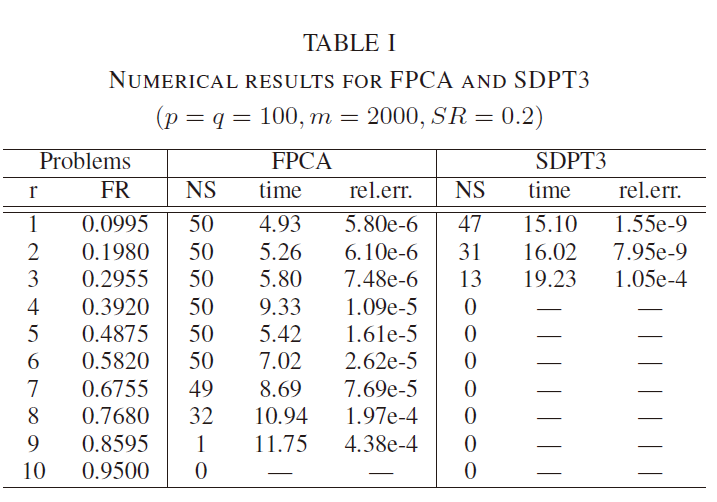
\includegraphics[width=10cm,height=7cm]{src//1.png}
            \end{frame}
            %--- Next Frame ---%
            \begin{frame}[t]{FPCA对比SVT(简单情况)}
                \centering
                    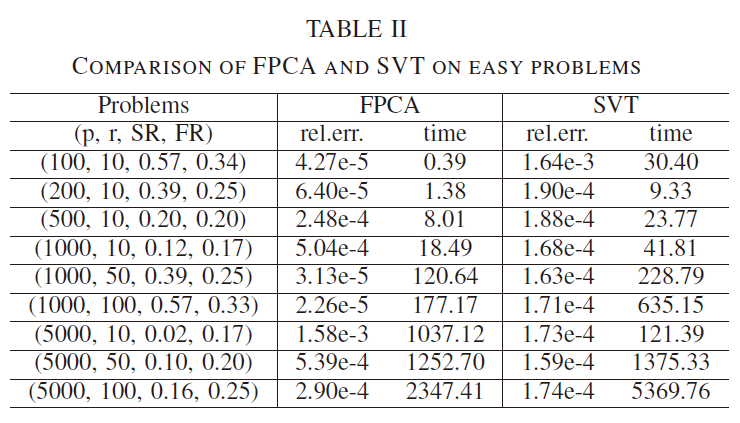
\includegraphics[width=10cm,height=6cm]{src//2.png}
            \end{frame}
            %--- Next Frame ---%
            \begin{frame}[t]{FPCA对比SVT(复杂情况)}
                \vspace{10mm}
                \centering
                    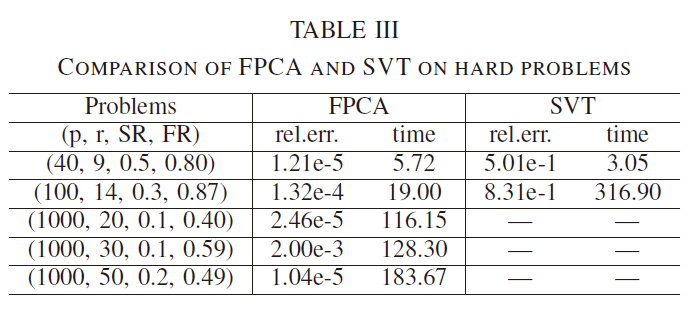
\includegraphics[width=10cm,height=5cm]{src//3.png}
            \end{frame}
            %--- Next Frame ---%
            \begin{frame}[t]{RBR}
                \centering
                    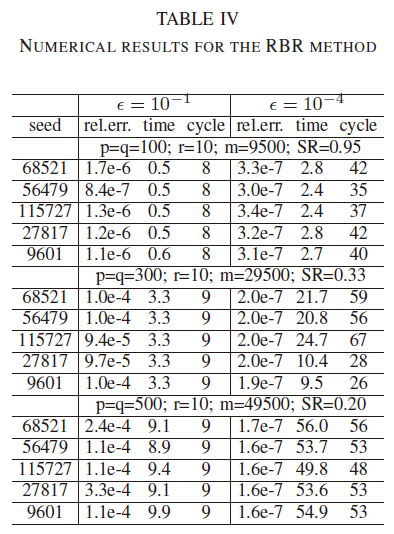
\includegraphics[width=5cm,height=7cm]{src//4.png}
            \end{frame}
            %--- Next Frame ---%
    %--- End Frame ---%
    \section*{End}                              %结束章节, 不列入目录
        \begin{frame}
            \vspace{35mm}                       %垂直距离
            %\hspace{10mm}                      %水平距离
            \centering                          %居中
                
\includegraphics{src//Thanks.pdf}    %插入图片
        \end{frame}
\end{document}                                  %结束正文
